\section{Keterampilan Pemrograman}
\begin{enumerate}
    \item Jawaban soal nomor 1
     \begin{figure}[!htbp]
        \centering
        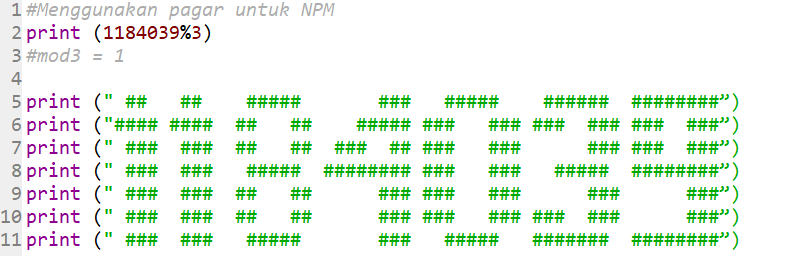
\includegraphics[width=10cm]{figures/pagarnpm.PNG}
        \caption{Nomor1}
    \end{figure}
    
     \item Jawaban soal nomor 2
     \begin{figure}[!htbp]
        \centering
        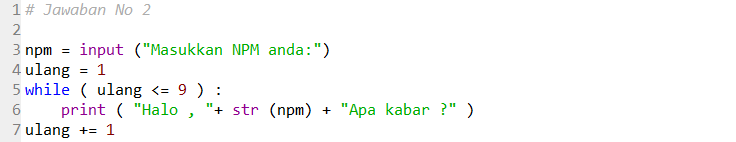
\includegraphics[width=12cm]{figures/jwb2.PNG}
        \caption{Nomor2}
    \end{figure}
    
     \item Jawaban soal nomor 3
     \begin{figure}[!htbp]
        \centering
        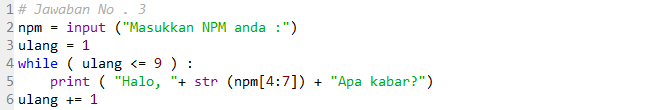
\includegraphics[width=12cm]{figures/jwb3.PNG}
        \caption{Nomor3}
    \end{figure}
    
     \item Jawaban soal nomor 4
     \begin{figure}[!htbp]
        \centering
        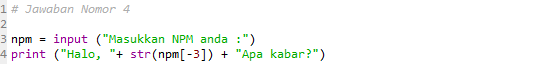
\includegraphics[width=15cm]{figures/jwb4.PNG}
        \caption{Nomor4}
    \end{figure}
    
    \newpage
     \item Jawaban soal nomor 5
     \begin{figure}[!htbp]
        \centering
        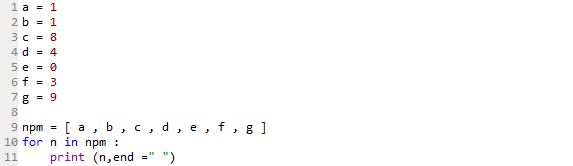
\includegraphics[width=12cm]{figures/jwb5.PNG}
        \caption{Nomor5}
    \end{figure}
    
     \item Jawaban soal nomor 6
     \begin{figure}[!htbp]
        \centering
        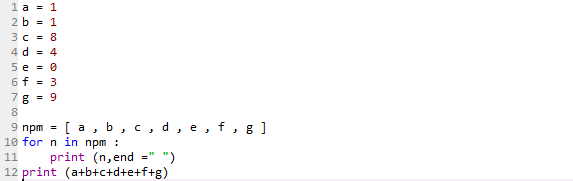
\includegraphics[width=12cm]{figures/jwb6.PNG}
        \caption{Nomor6}
    \end{figure}
    
     \item Jawaban soal nomor 7
     \begin{figure}[!htbp]
        \centering
        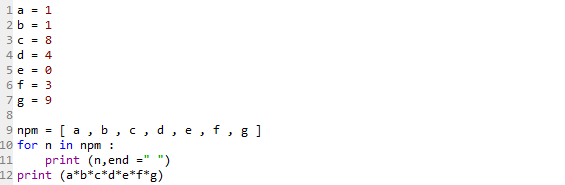
\includegraphics[width=12cm]{figures/jwb7.PNG}
        \caption{Nomor7}
    \end{figure}

\newpage
     \item Jawaban soal nomor 8
     \begin{figure}[!htbp]
        \centering
        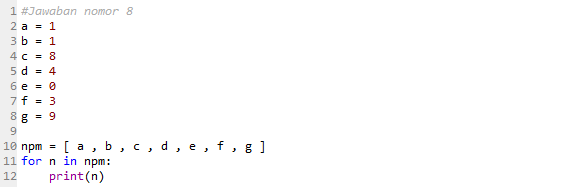
\includegraphics[width=12cm]{figures/jwb8.PNG}
        \caption{Nomor8}
    \end{figure}
    
     \item Jawaban soal nomor 9
     \begin{figure}[!htbp]
        \centering
        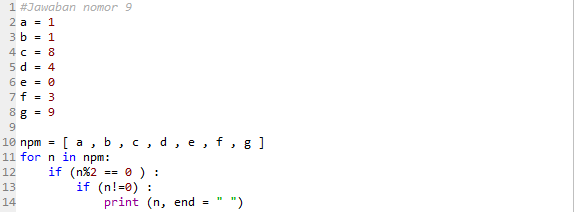
\includegraphics[width=12cm]{figures/jwb9.PNG}
        \caption{Nomor9}
    \end{figure}
    
     \item Jawaban soal nomor 10
     \begin{figure}[!htbp]
        \centering
        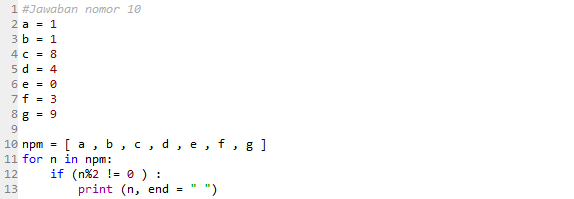
\includegraphics[width=12cm]{figures/jwb10.PNG}
        \caption{Nomor10}
    \end{figure}
    \newpage
     \item Jawaban soal nomor 11
     \begin{figure}[!htbp]
        \centering
        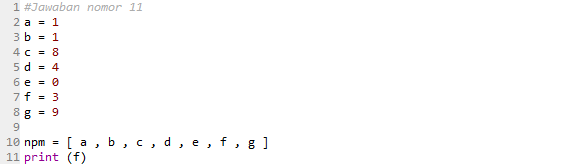
\includegraphics[width=15cm]{figures/jwb11new.PNG}
        \caption{Nomor11}
    \end{figure}
\end{enumerate}
\section{Keterampilan Penanganan Error}
\subsection{Jenis-Jenis Error dan Penanganannya}
\begin{enumerate}
    \item Syntax Error
    Syntax error adalah suatu keadaan atau kondisi ketika ada kesalahan penulisan kode pada program python hal ini menyebabkan program tidak dapat dijalankan. contohnya kesalahan pemberian titik dua atau tanda kutip. Output pemberitahuan error nya yaitu invalid syntax. Yang harus dilakukan saat terjadi syntax error pada kode program yaitu memperbaiki penulisan kodenya.
    \item Name Error
    Name error, yaitu exception yang muncul ketika melakukan eksekusi pada suatu program terhadapa lokal name dan global name tidak terdefinisi. error ini terjadi saat pemanggilan variabel yang tidak di definisikan atau memnaggil sebuah function yang tidak ada. Output pemberitahuan error nya yaitu name 'a' is not defined. Untuk mengatasi terjadi name error yaitu dengan memastikan variabel dan function yang akan dipanggil benar-benar ada dalam kode program dan tidak terjadi kesalahan penulisan.
    \item Type Error
    Type Error, yaitu suatu keadaan yang terjadi ketika melakukan eksekusi pada suatu operasi atau fungsi yang tipe datanya berbeda atau tidak sesuai dengan operasi yang akan dilakukan. Contoh kasusnya pada kesalahan tipe data antara string dan integer, kesalahan dalam input list,tupl dan dictionary. Cara penanganannya yaitu dengan mengkorversi variabel yang digunakan sesuai dengan tipe datanya.
    \item Identation error
    Identation error, yaitu tulisasn kode program yang menjorok. identation error akan terjadi ketika mengetik kode program namun tidak memperhatikan identasinya. Jika terjadi identasi maka program akan error. cara mengatasinya yaitu memperhatikan identasi saat menuliskan suatu program.
\end{enumerate}
\subsection{Penanganan Error}
     \begin{figure}[!htbp]
        \centering
        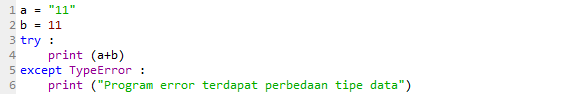
\includegraphics[width=15cm]{figures/jwb12.PNG}
        \caption{Penanganan Error}
    \end{figure}
